\addcontentsline{toc}{section}{\hspace{17pt}Appendix} % Adds to the Table of contents
\section*{Appendix}
\renewcommand*\thesubsection{\Roman{subsection}} % Makes all subsections be listed with upper case roman numbers
\subsection{Illustrations} \label{illustrations}

\textbf{[ TODO: Make tables and images have same width. Also update the header to say "Appendix" instead of "References". ]}

\begin{figure}[H]
  \centering
  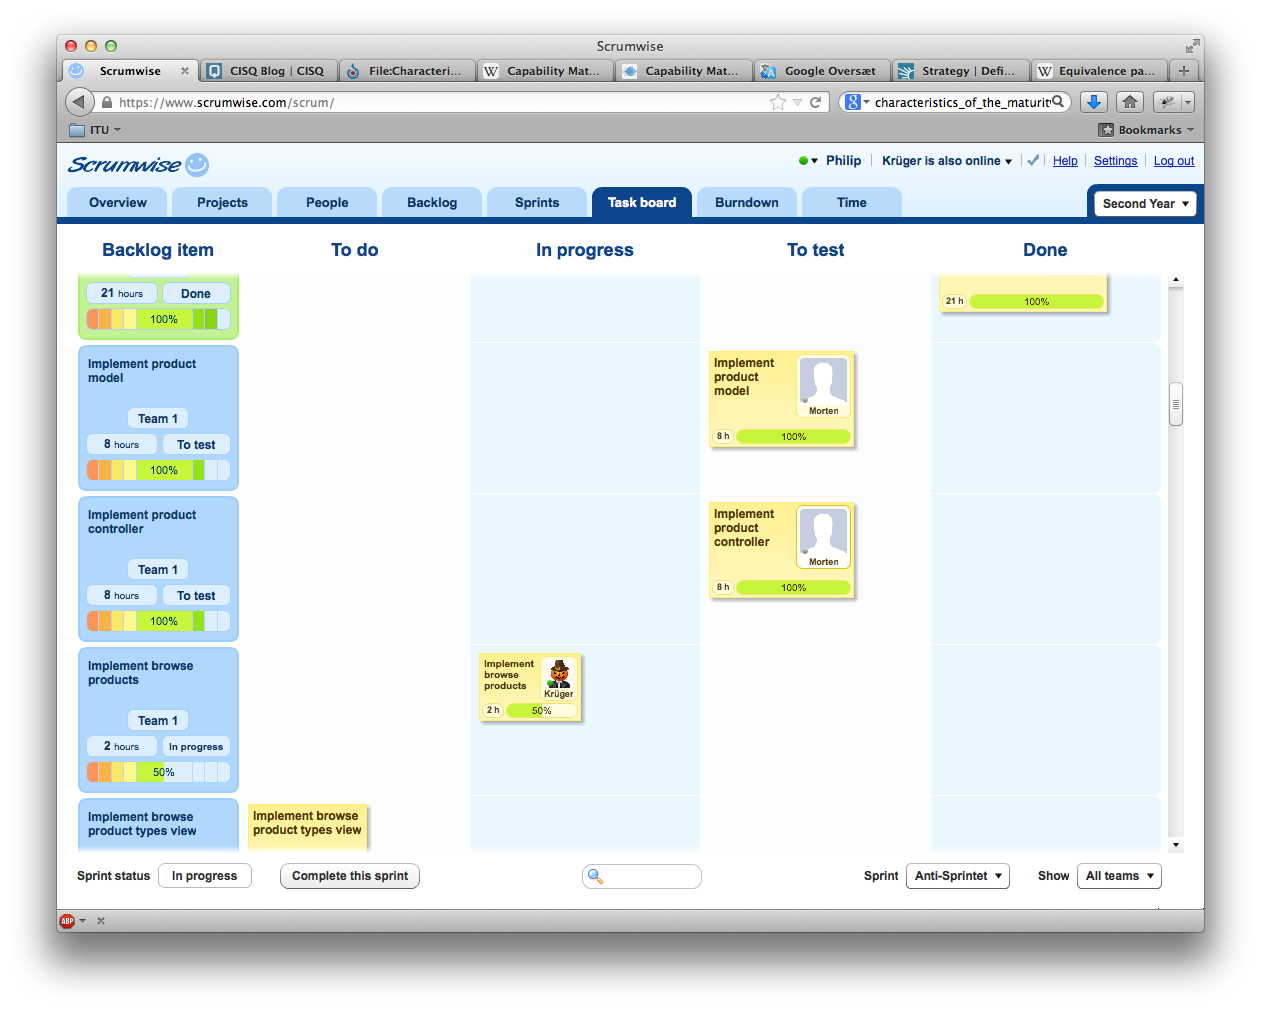
\includegraphics[width=\textwidth]{illustrations/taskboard}
  \caption{Taskboard.}
  \label{taskboard}
\end{figure}

\begin{figure}[H]
  \centering
  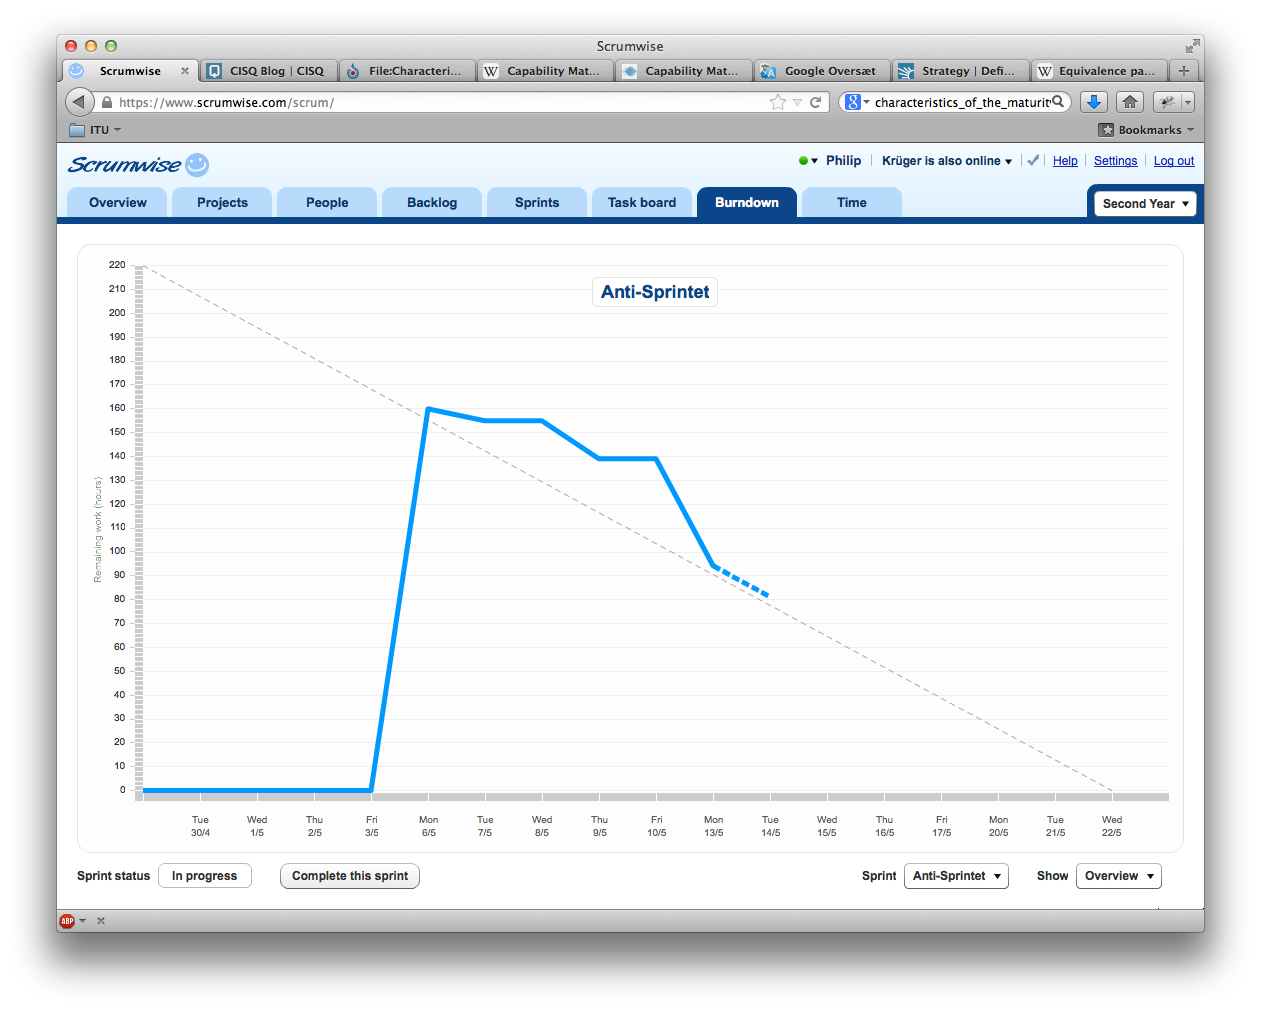
\includegraphics[width=\textwidth]{illustrations/burndown}
  \caption{Burndown chart. At the point of writing it seems like we are on track.}
  \label{burndown}
\end{figure}

% BACKLOG TABLE START %
\begin{longtable}{|p{200px}|p{200px}|}
\caption[Backlog]{Backlog} \label{backlog} \\

\hline \multicolumn{1}{|c|}{\textbf{Time (s)}} & \multicolumn{1}{c|}{\textbf{Description}} \\
\endfirsthead

\multicolumn{2}{c}%
{{\bfseries \tablename\ \thetable{} -- continued from previous page}} \\
\hline \multicolumn{1}{|c|}{\textbf{Name (s)}} &
\multicolumn{1}{c|}{\textbf{Description}} \\ \hline 
\endhead

\hline %\multicolumn{3}{|r|}{{Continued on next page}} \\ \hline
\endfoot

\hline
\endlastfoot
    \hline
	Convert API images to spreadsheet & ~  \\
	\hline
		Create diagrams & Class diagrams, SSD, Design mockups (if time), Package diagram, etc. \\ \hline
	Program structure & Create repository, files and empty methods from the interface \\ \hline
	Implement composite structure base classes & ~ \\ \hline
	Implement JSON class & ~  \\ \hline
	Implement web-service class & ~ \\ \hline
	Implement page view & ~  \\ \hline
	Implement base functionality for views & Slide out, Click field to edit, Fixed header, Ajax mouseover to view, Buttons, Fields,	etc. \\ \hline
	Implement product model & ~  \\ \hline
	Implement product controller & ~  \\ \hline
	Implement browse products & ~  \\ \hline
	Implement browse product types view & ~  \\
	Implement auth model & ~  \\ \hline
	Implement auth controller & ~  \\ \hline
	Implement login/create widget in header & ~  \\ \hline
	Implement logged-in mouseover in header view & ~  \\ \hline	
	Implement single dropdown autocomplete widget & ~  \\ \hline
	Implement multiple dropdown autocomplete widget & ~  \\ \hline
	Implement product view & ~  \\ \hline
	Implement rating widget view & ~  \\ \hline
	Implement purchases model & ~  \\ \hline
	Implement purchases controller & ~  \\ \hline
	Implement buy/rent widget view & ~  \\ \hline
	Implement stream view & ~  \\ \hline
	Implement credits model & ~  \\ \hline
	Implement credits controller & ~  \\ \hline
	Implement account model & ~  \\ \hline
	Implement account controller & ~  \\ \hline
	Implement account profile view & ~  \\ \hline
	Implement purchases view & ~  \\ \hline
	Implement customer dashboard view & ~  \\ \hline
	Implement content provider dashboard view & ~  \\ \hline
	Implement search products view & ~  \\ \hline
	Implement browse accounts view & ~  \\ 
	Test WCF Service Controllers & Helper Classes needs to be refactored to use interfaces. Mockup implementations needs to be made. \\ \hline
	Define Report Structure & ~  \\ \hline
	Write Introduction & ~  \\ \hline
	Write Problem statement and requirements & ~  \\ \hline
	Write Use Cases & Server and client  \\ \hline
	Write Software Analysis (server) & Why have we chosen the technologies we have? \\ \hline
	Write Software Design and architecture (server) & ~  \\ \hline
	Write Testing (server) & ~  \\ \hline
	Write Software Analysis (client) & ~  \\ \hline
	Write Software Design and architecture (client) & ~  \\ \hline
	Write Testing (client) & ~  \\ \hline
	Write Conclusion & ~  \\ \hline
	Write Abstract & ~  \\ \hline
\end{longtable}
\newpage

\begin{landscape}
\begin{figure}[H]
  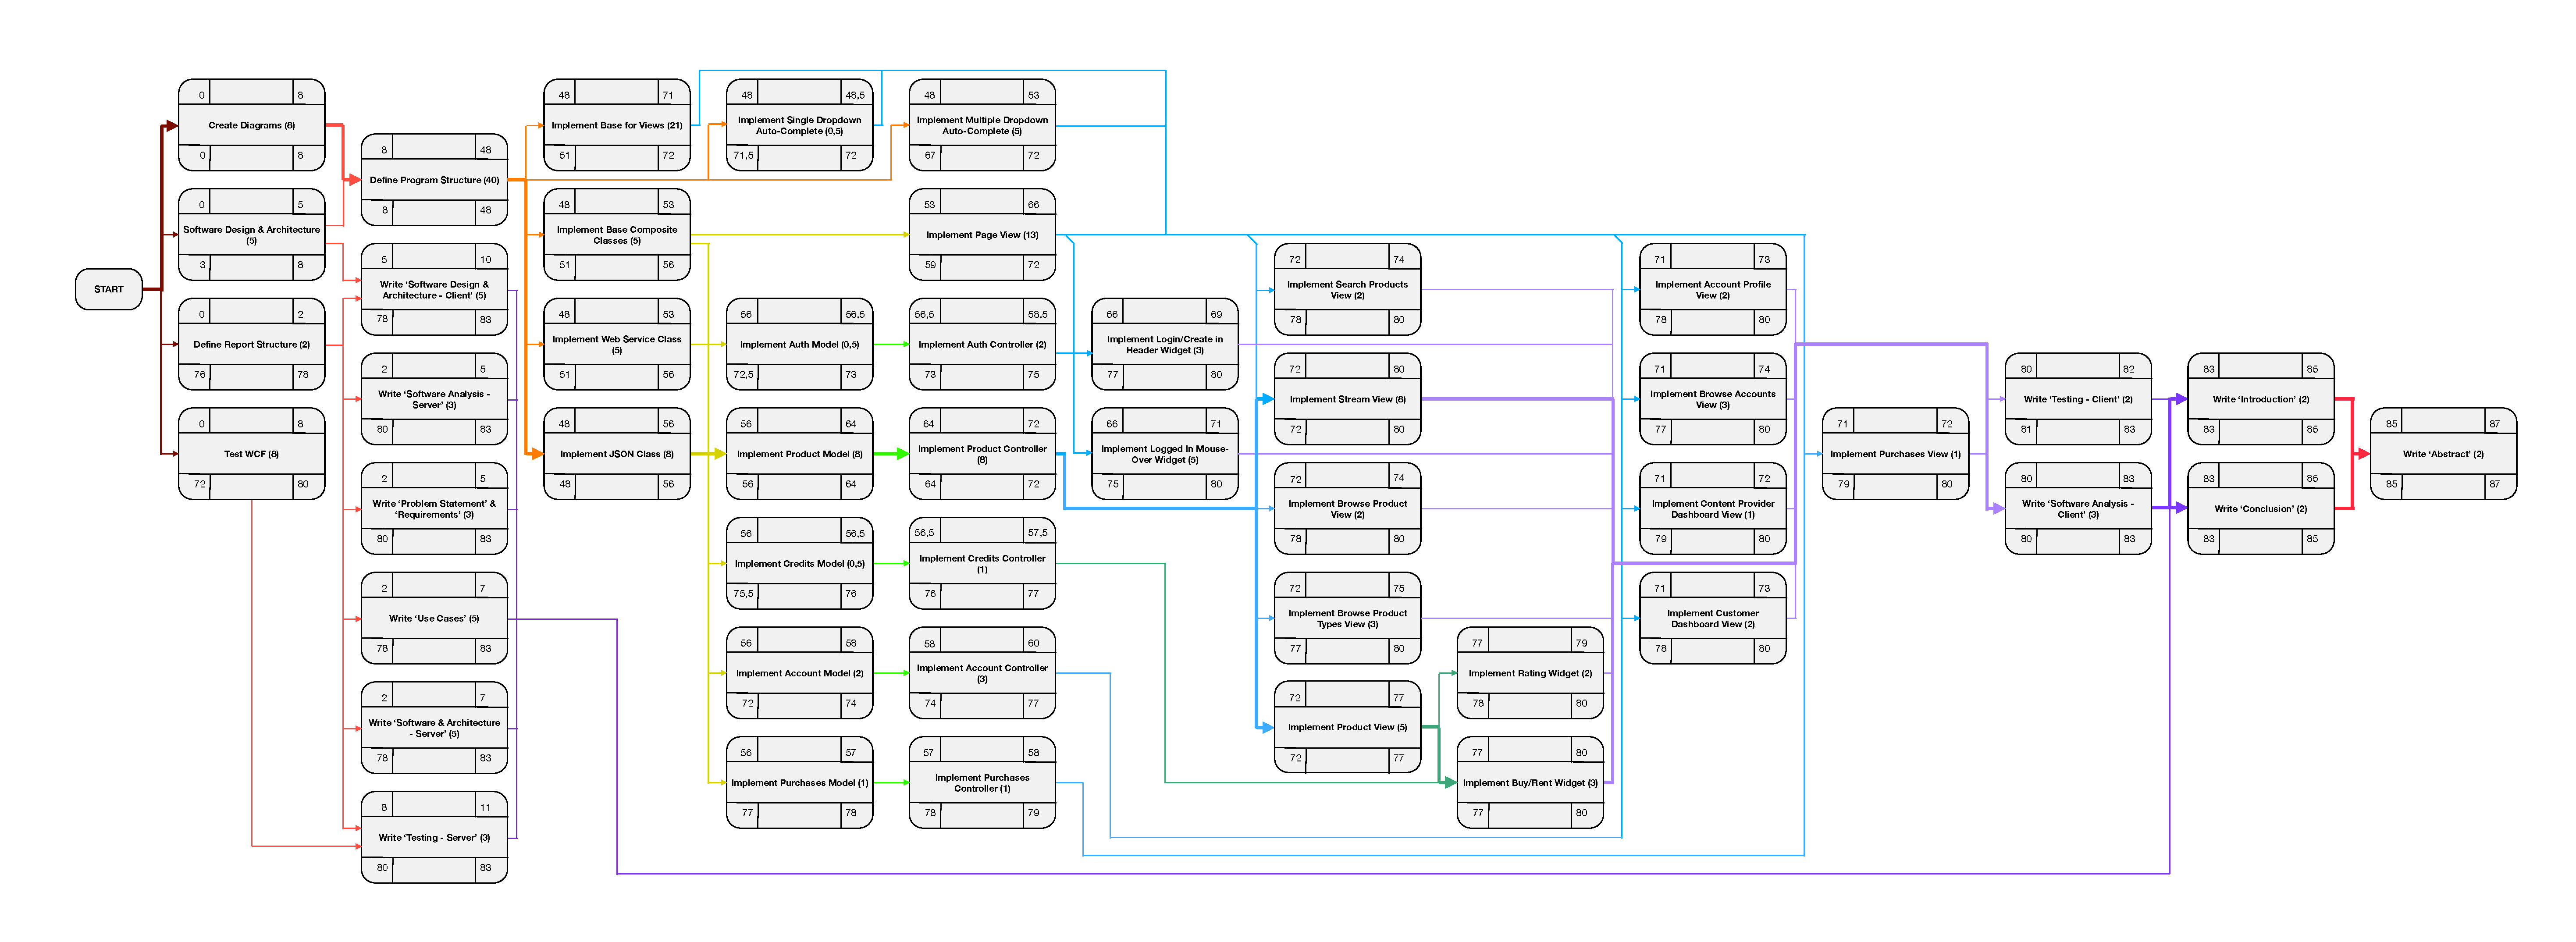
\includepdf[landscape]{illustrations/Dependency_network.pdf}
  \caption{Dependency network}
  \label{dependency_network}
\end{figure}
\end{landscape}

\newpage
\renewcommand{\section}[2]{} % Removing some bug where it added a heading after this? :S